\section{Referencia de la Clase List\-Lin\-Albaran\-Cliente\-View}
\label{classListLinAlbaranClienteView}\index{ListLinAlbaranClienteView@{ListLinAlbaranClienteView}}
Muestra y administra las l\'{\i}neas de detalle de albaranes a un cliente.  


{\tt \#include $<$listlinalbaranclienteview.h$>$}

Diagrama de herencias de List\-Lin\-Albaran\-Cliente\-View\begin{figure}[H]
\begin{center}
\leavevmode
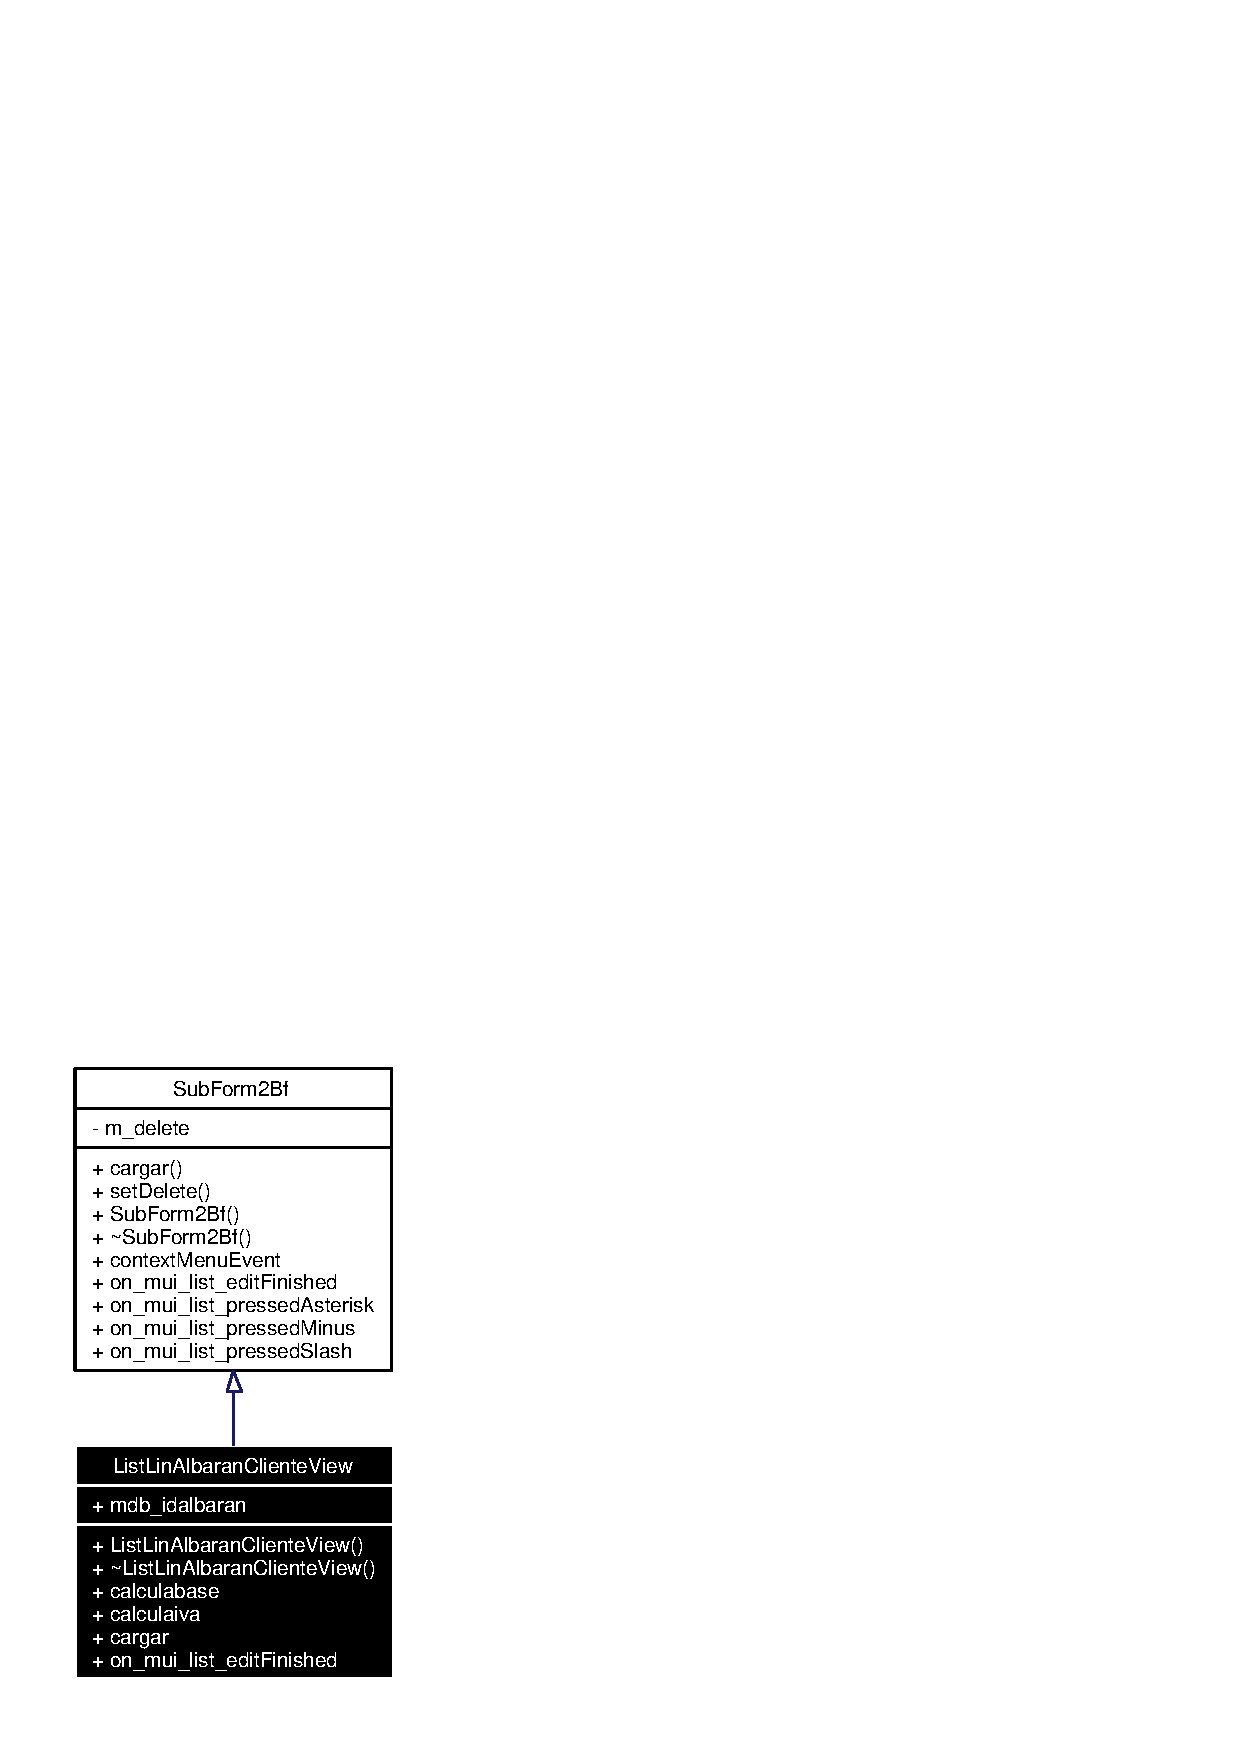
\includegraphics[width=94pt]{classListLinAlbaranClienteView__inherit__graph}
\end{center}
\end{figure}
Diagrama de colaboraci\'{o}n para List\-Lin\-Albaran\-Cliente\-View:\begin{figure}[H]
\begin{center}
\leavevmode
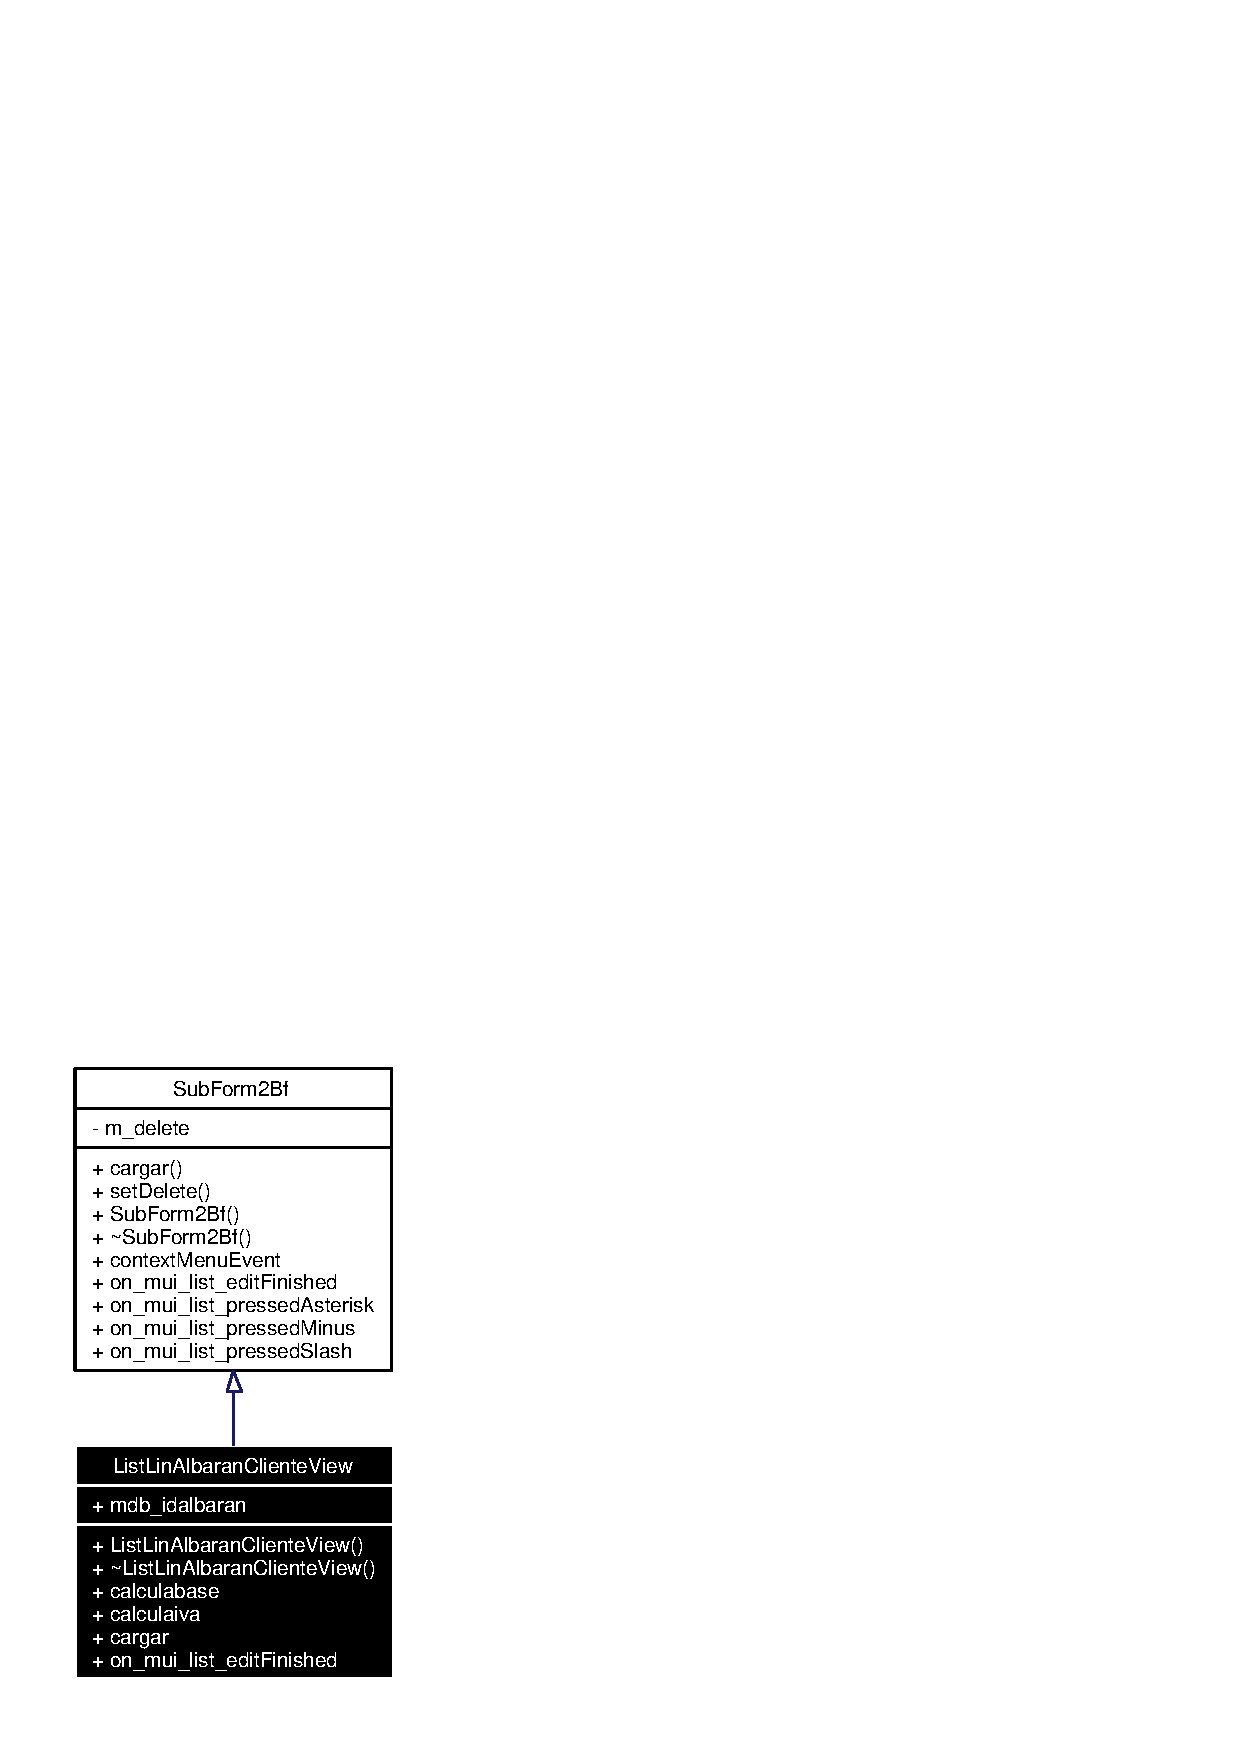
\includegraphics[width=94pt]{classListLinAlbaranClienteView__coll__graph}
\end{center}
\end{figure}
\subsection*{Slots p\'{u}blicos}
\begin{CompactItemize}
\item 
Fixed {\bf calculabase} ()\label{classListLinAlbaranClienteView_i0}

\item 
Fixed {\bf calculaiva} ()\label{classListLinAlbaranClienteView_i1}

\item 
virtual void {\bf cargar} (QString idalbaran)\label{classListLinAlbaranClienteView_i2}

\item 
virtual void {\bf on\_\-mui\_\-list\_\-edit\-Finished} (int, int)\label{classListLinAlbaranClienteView_i3}

\end{CompactItemize}
\subsection*{M\'{e}todos p\'{u}blicos}
\begin{CompactItemize}
\item 
{\bf List\-Lin\-Albaran\-Cliente\-View} (QWidget $\ast$parent=0)\label{classListLinAlbaranClienteView_a0}

\end{CompactItemize}
\subsection*{Atributos p\'{u}blicos}
\begin{CompactItemize}
\item 
QString {\bf mdb\_\-idalbaran}\label{classListLinAlbaranClienteView_o0}

\end{CompactItemize}


\subsection{Descripci\'{o}n detallada}
Muestra y administra las l\'{\i}neas de detalle de albaranes a un cliente. 



La documentaci\'{o}n para esta clase fu\'{e} generada a partir de los siguientes archivos:\begin{CompactItemize}
\item 
listlinalbaranclienteview.h\item 
listlinalbaranclienteview.cpp\end{CompactItemize}
